\documentclass[14pt,pdf,hyperref={unicode}]{beamer}

% \documentclass[aspectratio=43]{beamer}
% \documentclass[aspectratio=1610]{beamer}
% \documentclass[aspectratio=169]{beamer}

\usepackage{lmodern}

% подключаем кириллицу 
\usepackage[T2A]{fontenc}
\usepackage[utf8]{inputenc}
\usepackage{listings}
\usepackage{graphicx}
\usepackage{hyperref}

% отключить клавиши навигации
\setbeamertemplate{navigation symbols}{}

% тема оформления
\usetheme{CambridgeUS}

% цветовая схема
\usecolortheme{seahorse}

\definecolor{light-gray}{gray}{0.90}

\lstset{basicstyle=\ttfamily,breaklines=true}

\title{Семинар №9}   
\subtitle{ФАКИ 2015}
\author{Бирюков В. А.} 
\date{\today} 
% \logo{
\includegraphics[height=5mm]{images/logo.png}\vspace{-7pt}}

\begin{document}

\lstset{language=C}

% титульный слайд
\begin{frame}
\titlepage
\end{frame} 

\defverbatim[colored]\makeset{
\begin{lstlisting}[language=C++,basicstyle=\ttfamily,keywordstyle=\color{blue}]
void make_set(int X) {
  parent[X] = X;
}
\end{lstlisting}
}

\lstset{
  language=C,                % choose the language of the code
  keywordstyle=\color{blue},
  numbers=none,                   % where to put the line-numbers
  stepnumber=1,                   % the step between two line-numbers.        
  numbersep=5pt,                  % how far the line-numbers are from the code
  backgroundcolor=\color{light-gray},  % choose the background color. You must add \usepackage{color}
  showspaces=false,               % show spaces adding particular underscores
  showstringspaces=false,         % underline spaces within strings
  showtabs=false,                 % show tabs within strings adding particular underscores
  tabsize=2,                      % sets default tabsize to 2 spaces
  captionpos=b,                   % sets the caption-position to bottom
  breaklines=true,                % sets automatic line breaking
  breakatwhitespace=true,         % sets if automatic breaks should only happen at whitespace
}








\section{Указатели}
\begin{frame}
\begin{center}
\begin{beamercolorbox}[sep=8pt,center]{part
title}
\usebeamerfont{part title}\insertsection
\end{beamercolorbox}
\end{center}
\end{frame}


\begin{frame}[fragile]
\frametitle{Указатели} 
\begin{itemize}
\item Указатель -- это переменная, содержащая адрес другой переменной.
\item Указатели и массивы тесно связаны между собой
\end{itemize}
\end{frame}


\begin{frame}[fragile]
\frametitle{Указатели} 
\framesubtitle{Указатели в памяти, объявление указателей}
\begin{center}
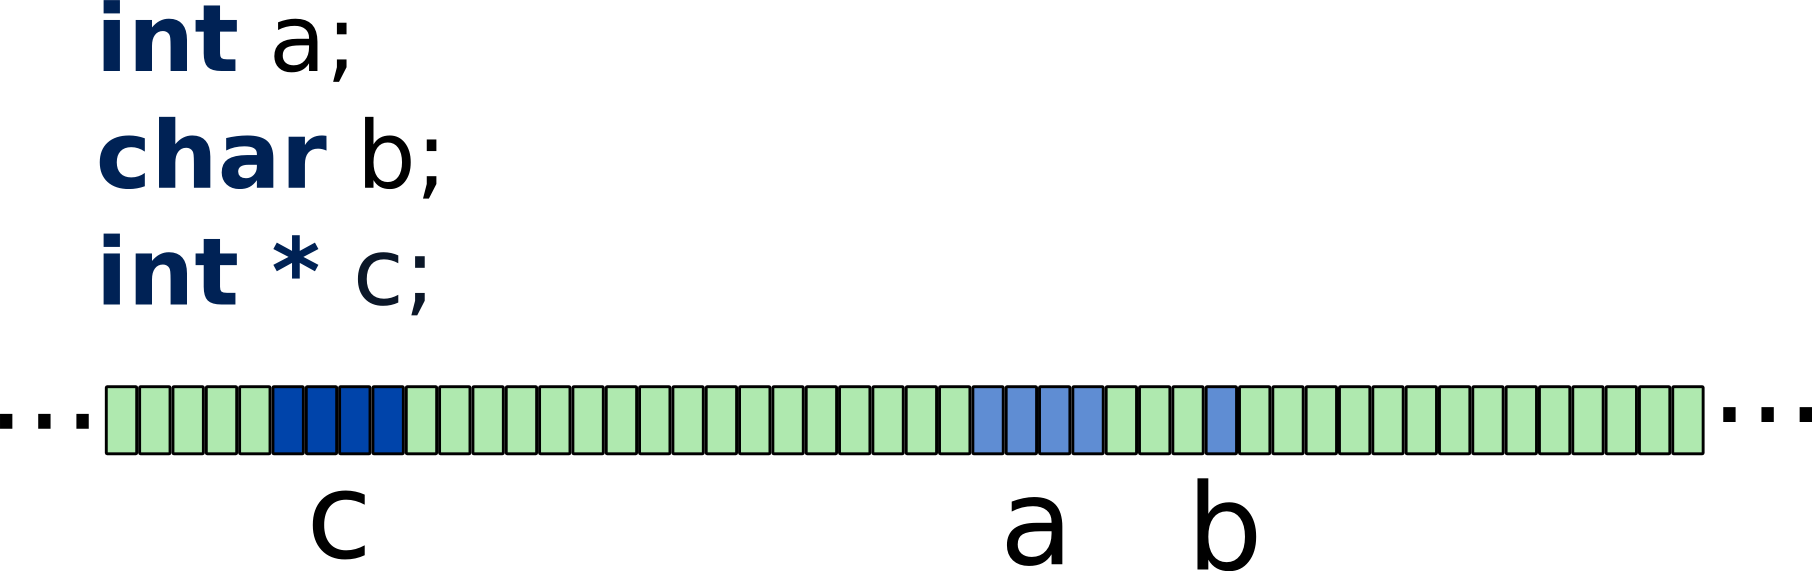
\includegraphics[width=0.95\linewidth]{images/memory_pointer_1.png}
\end{center}
\end{frame}

\begin{frame}[fragile]
\frametitle{Указатели} 
\framesubtitle{Адрес переменной}
\begin{center}
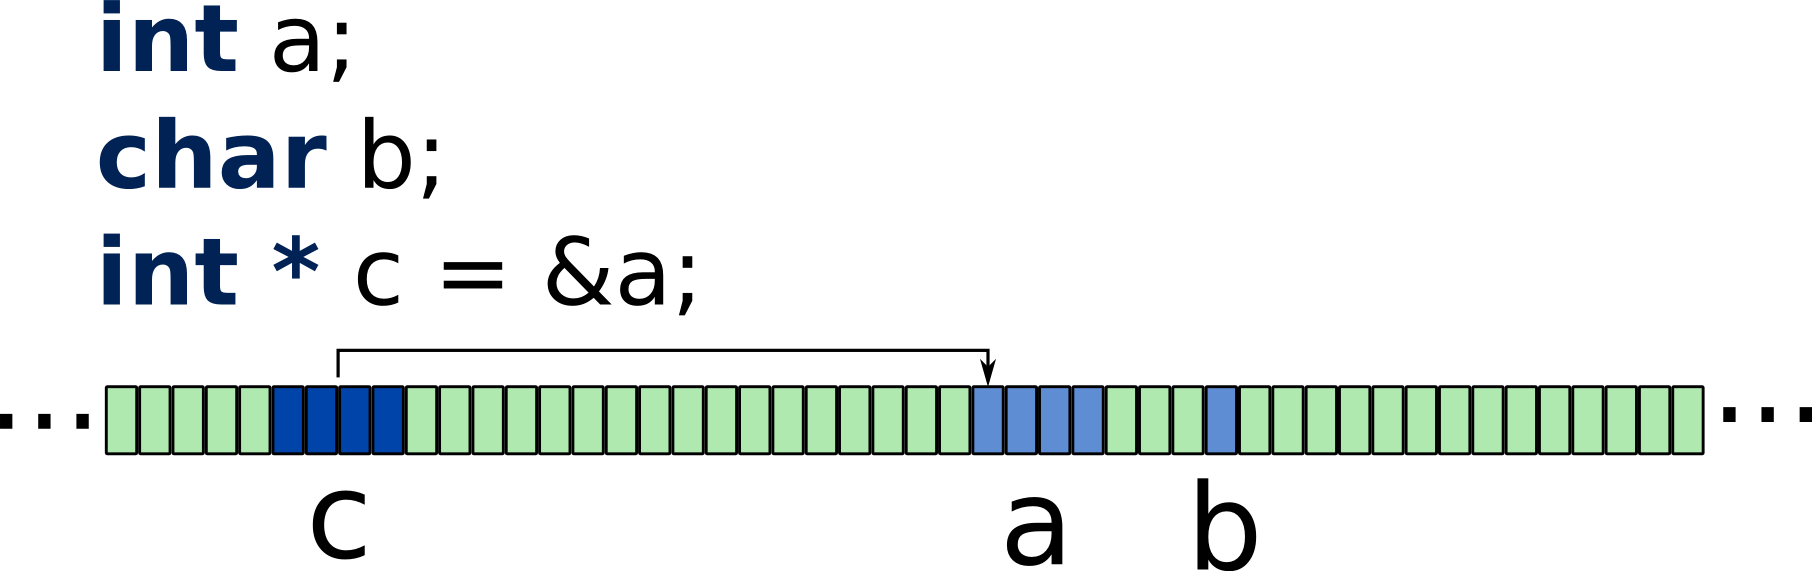
\includegraphics[width=0.95\linewidth]{images/memory_pointer_2.png}
\end{center}
\end{frame}

\begin{frame}[fragile]
\frametitle{Указатели} 
\framesubtitle{Адрес переменной}
\begin{center}
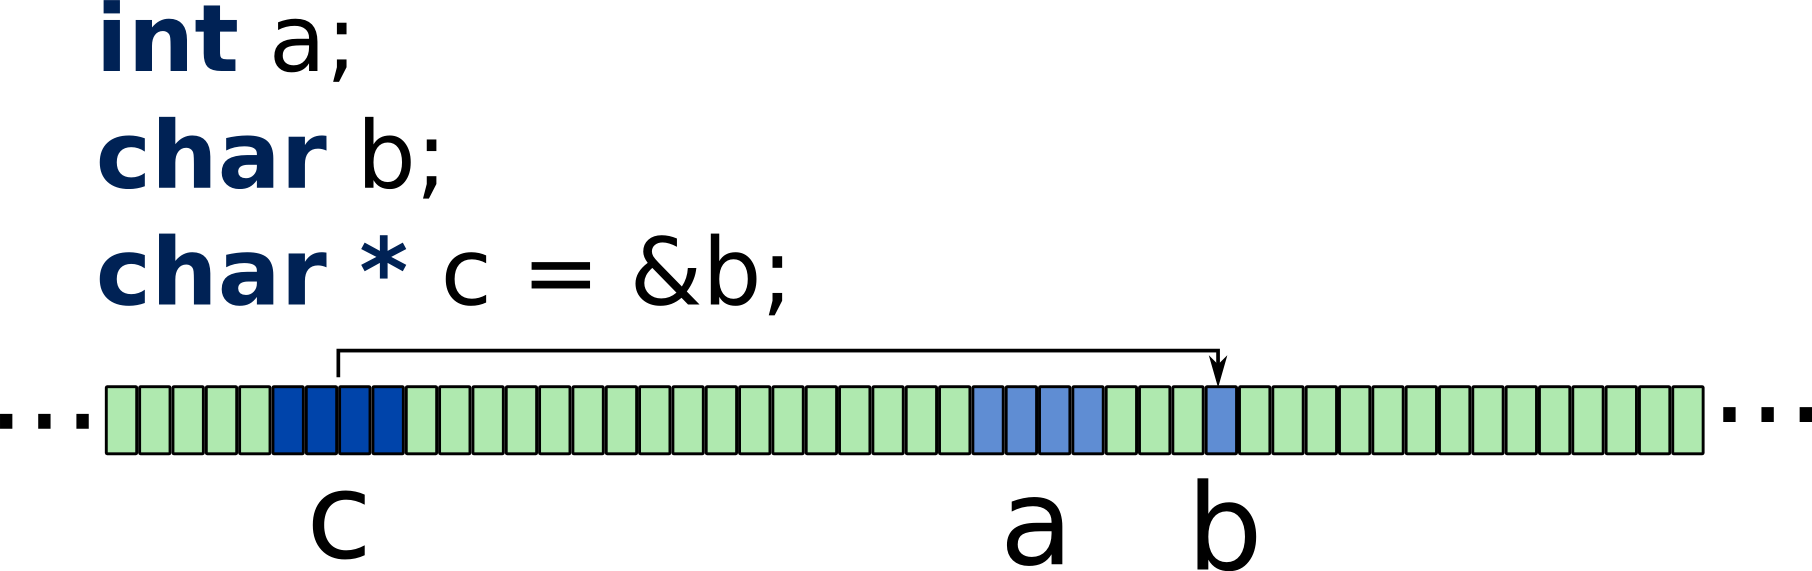
\includegraphics[width=0.95\linewidth]{images/memory_pointer_3.png}
\end{center}
\end{frame}

\begin{frame}[fragile]
\frametitle{Указатели} 
\framesubtitle{Ссылка по указателю}
\begin{center}
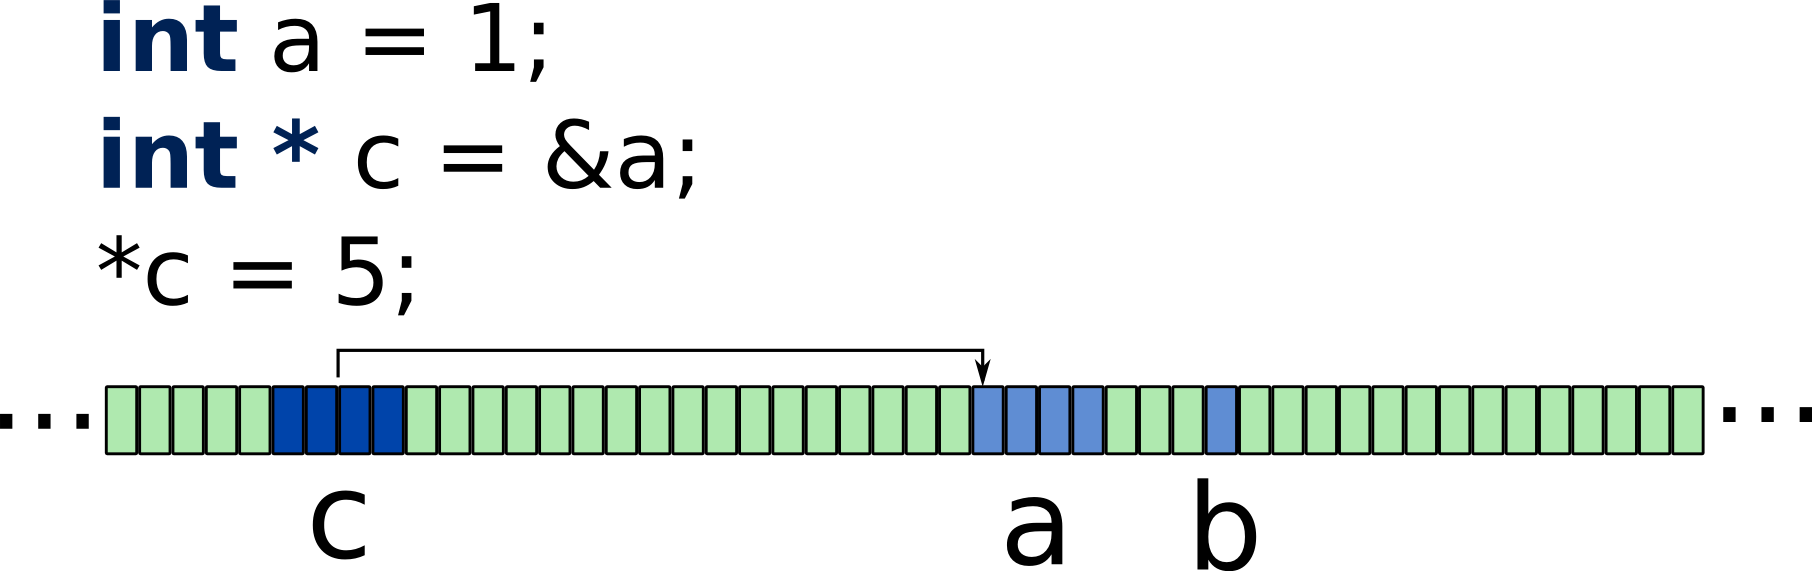
\includegraphics[width=0.95\linewidth]{images/memory_pointer_4.png}
\end{center}
\end{frame}


\section{Указатели и аргументы функций}
\begin{frame}
\begin{center}
\begin{beamercolorbox}[sep=8pt,center]{part
title}
\usebeamerfont{part title}\insertsection
\end{beamercolorbox}
\end{center}
\end{frame}

\begin{frame}[fragile]
\frametitle{Указатели и аргументы функций} 
\framesubtitle{Передача по значению}
\begin{center}
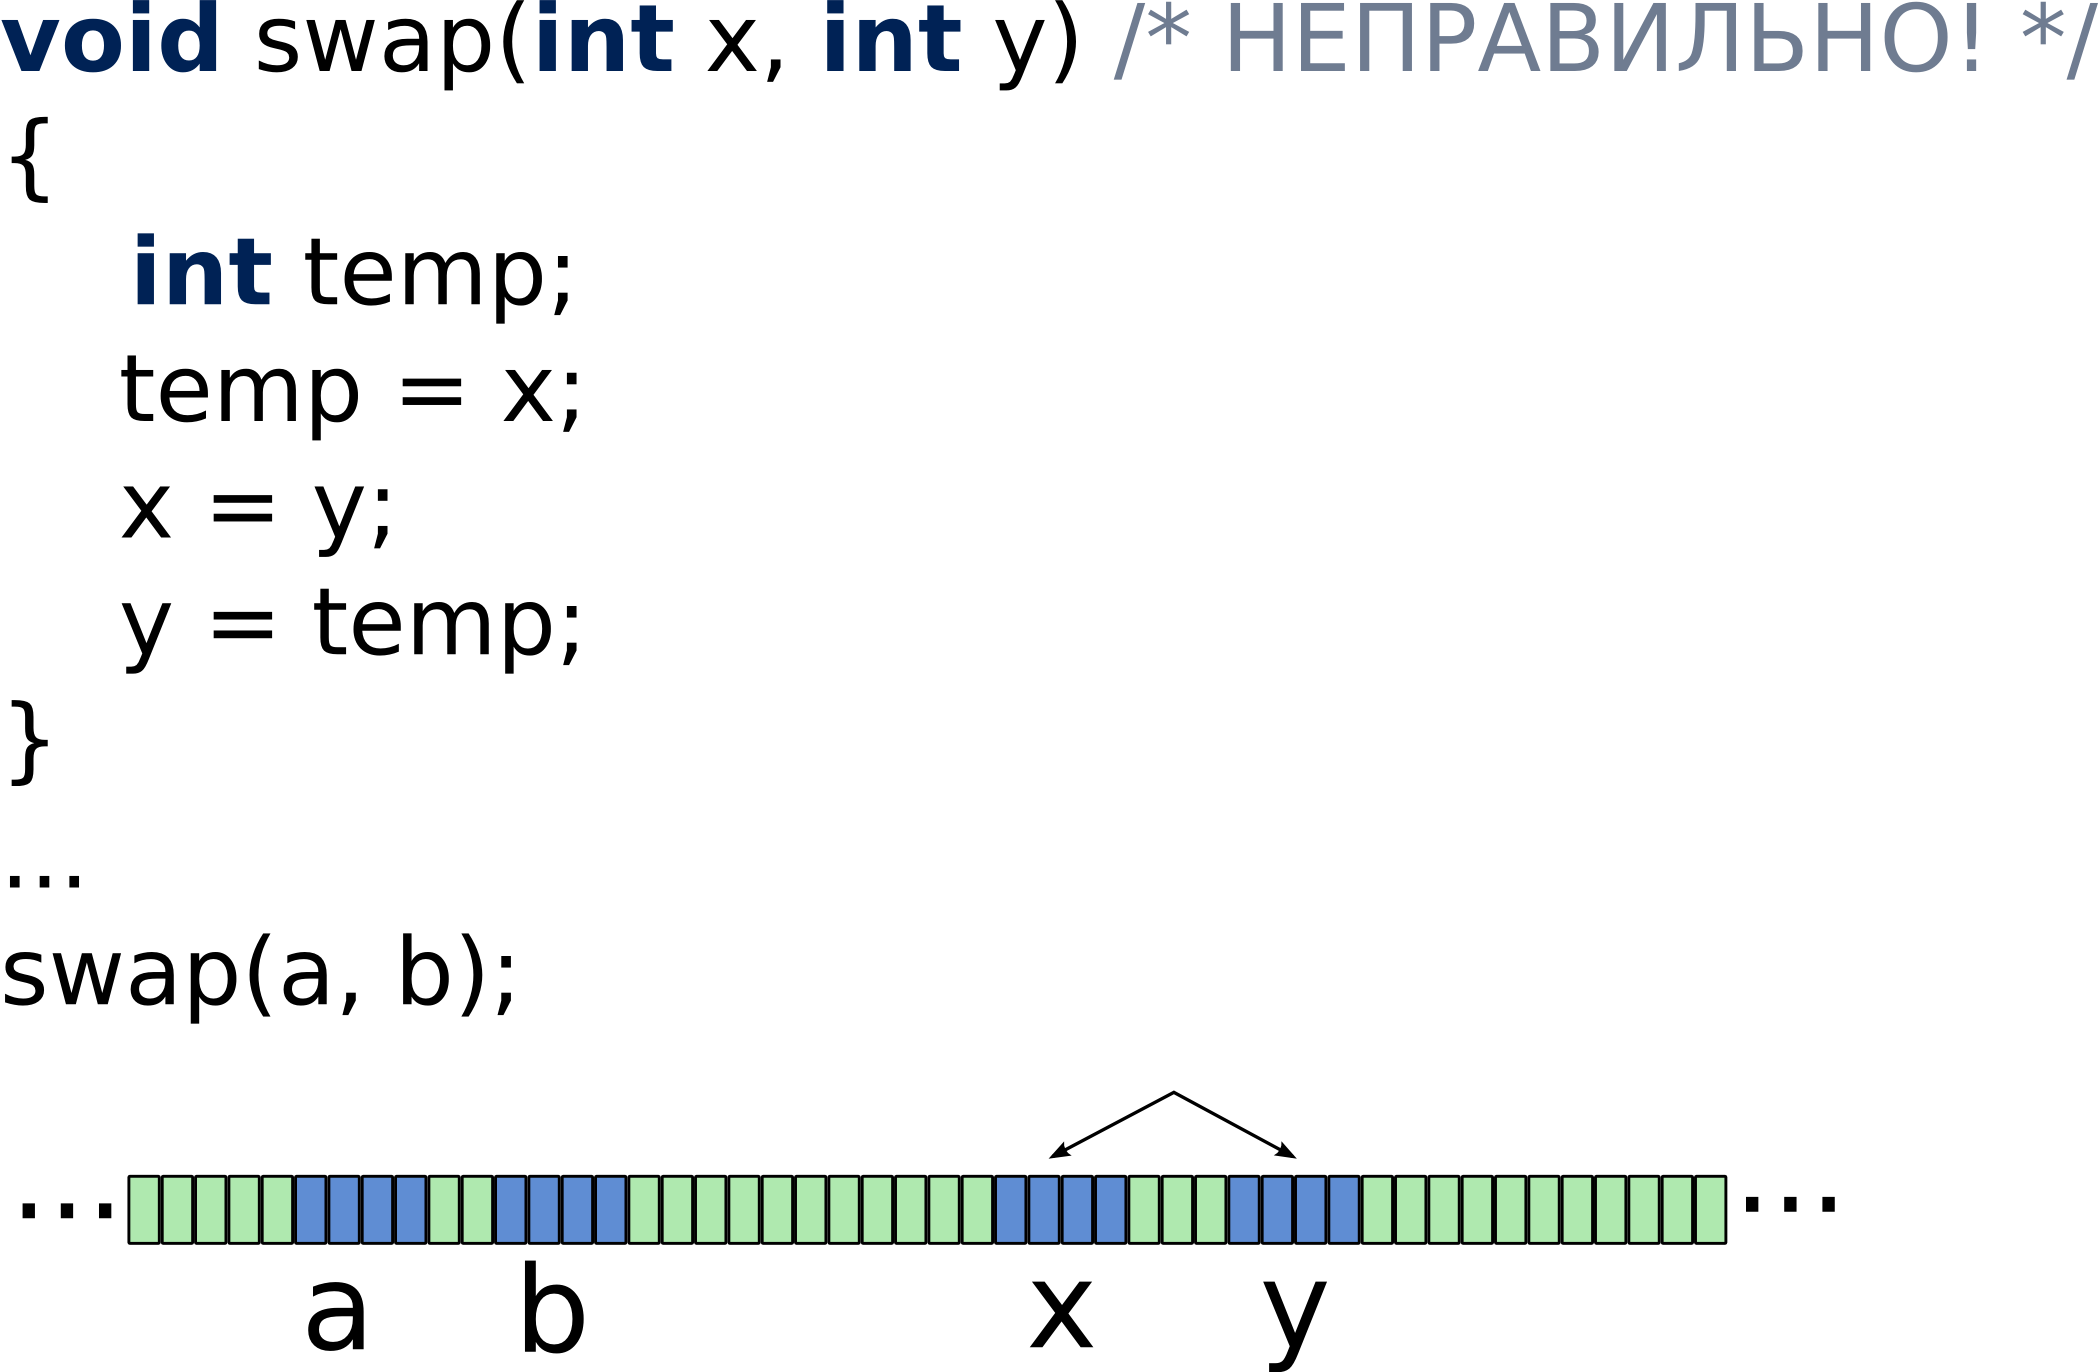
\includegraphics[height=0.55\linewidth]{images/swap_wrong.png}
\end{center}
\end{frame}

\begin{frame}[fragile]
\frametitle{Указатели и аргументы функций} 
\framesubtitle{Передача по адресу}
\begin{center}
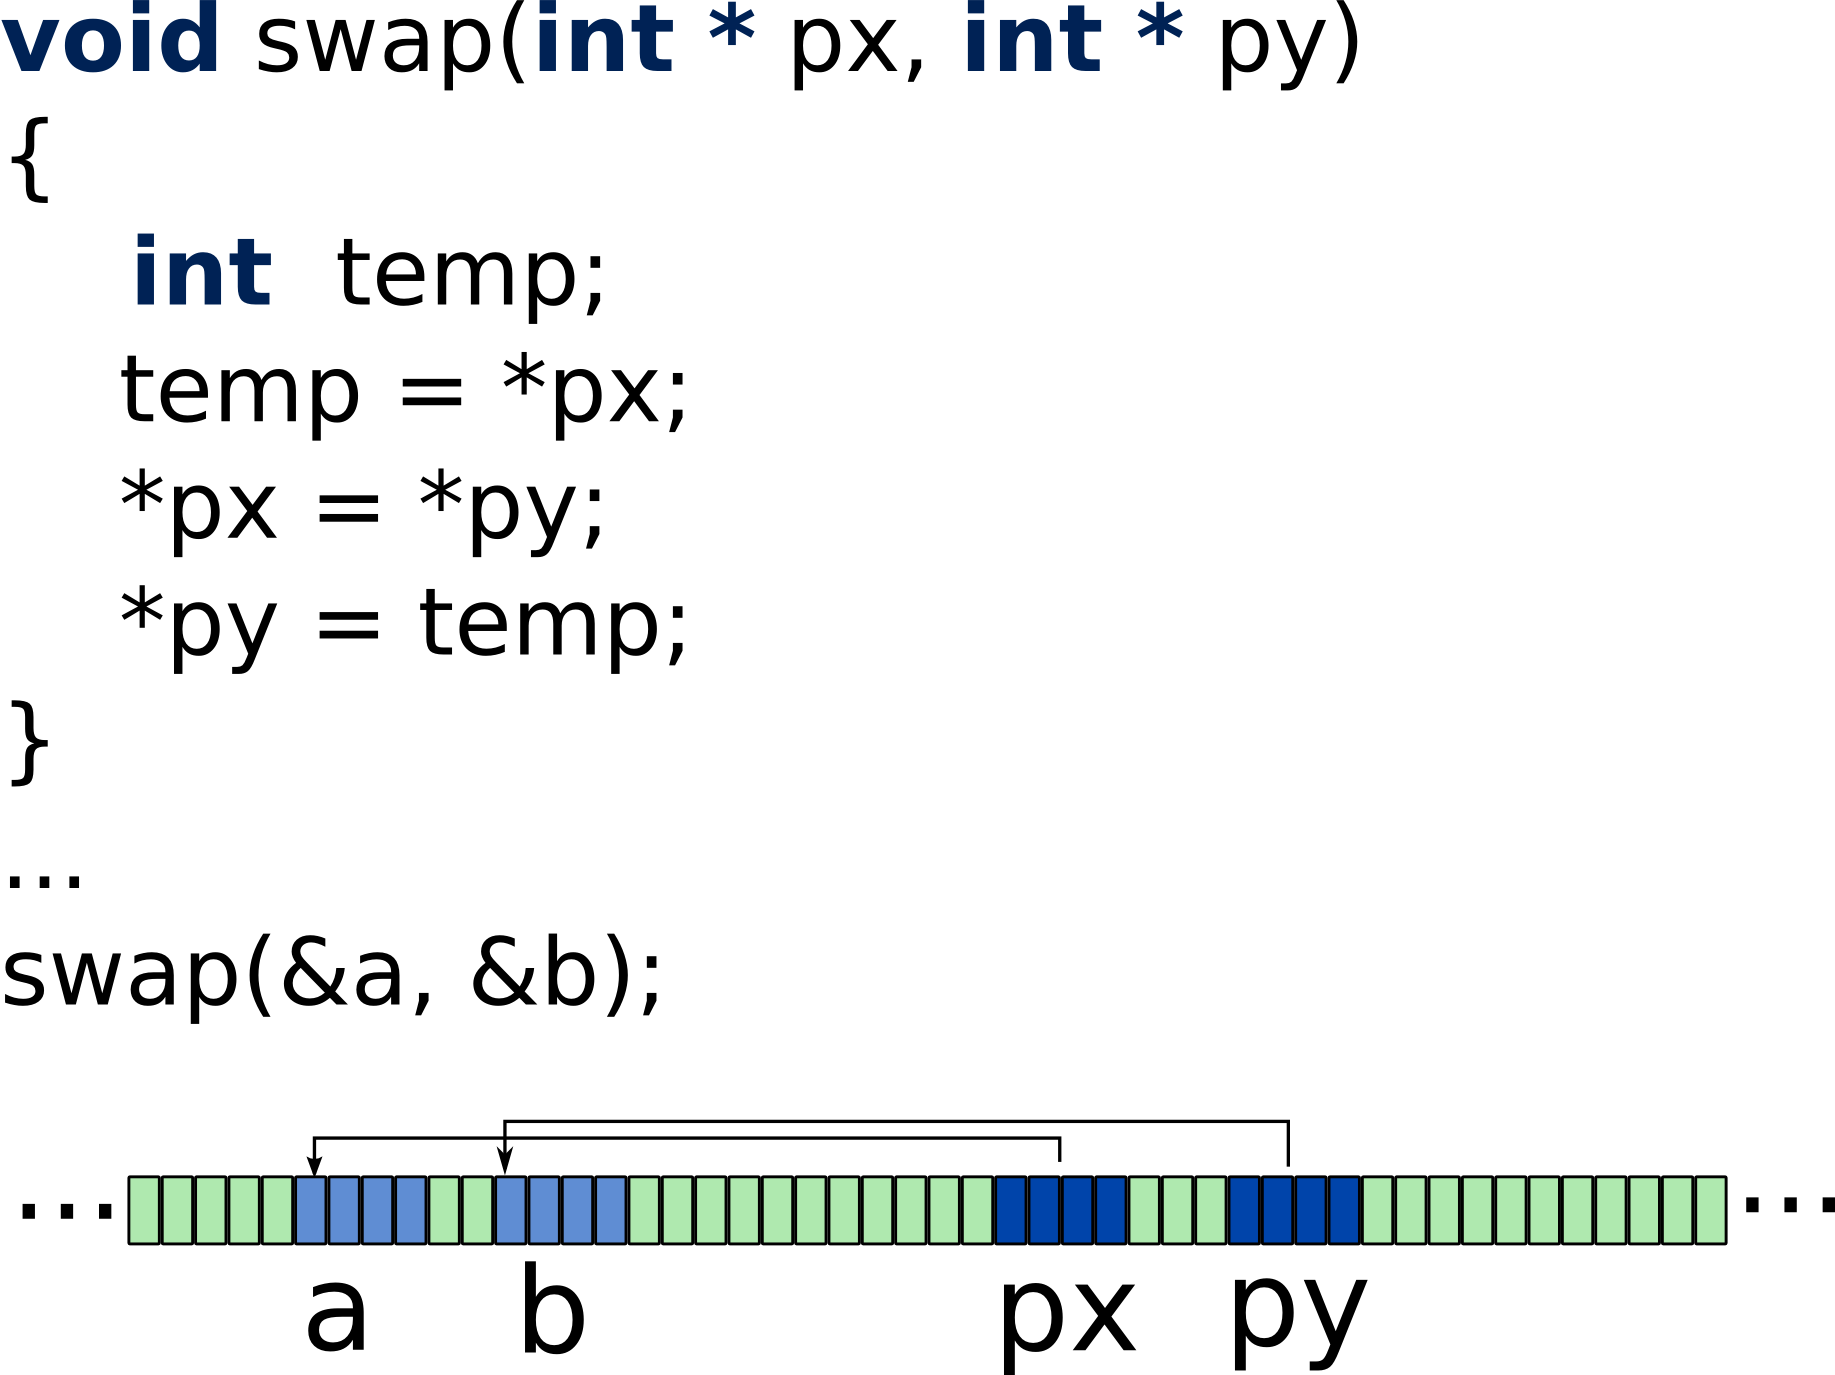
\includegraphics[height=0.55\linewidth]{images/swap_right.png}
\end{center}
\end{frame}


\section{Указатели и массивы}
\begin{frame}
\begin{center}
\begin{beamercolorbox}[sep=8pt,center]{part
title}
\usebeamerfont{part title}\insertsection
\end{beamercolorbox}
\end{center}
\end{frame}

\begin{frame}[fragile]
\frametitle{Указатели и массивы} 
\framesubtitle{Указатель на элемент массива}
\begin{center}
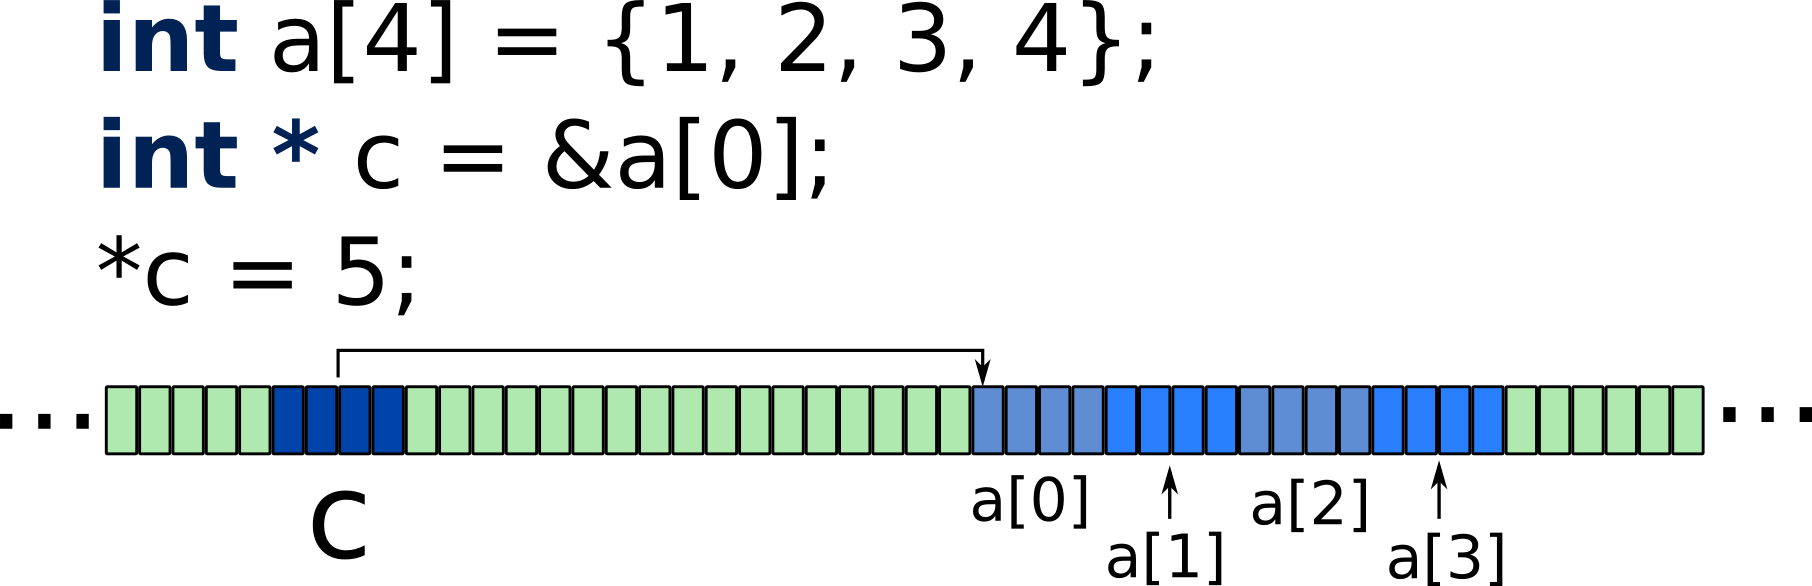
\includegraphics[width=0.95\linewidth]{images/memory_parrays_1.png}
\end{center}
\end{frame}

\begin{frame}[fragile]
\frametitle{Указатели и массивы} 
\framesubtitle{Адресная арифметика}
\begin{center}
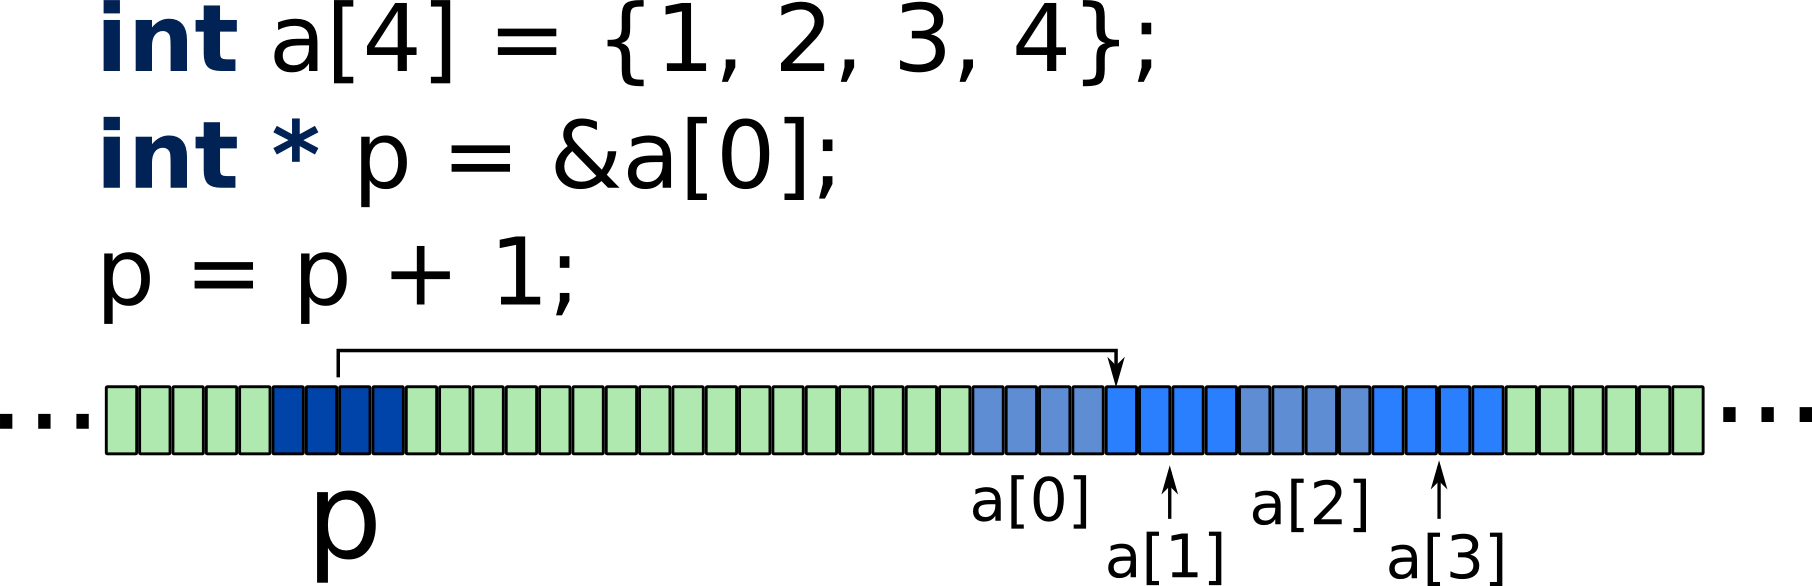
\includegraphics[width=0.95\linewidth]{images/memory_parrays_2.png}
\end{center}
\end{frame}

\begin{frame}[fragile]
\frametitle{Указатели и массивы} 
\framesubtitle{Адресная арифметика}
\begin{center}
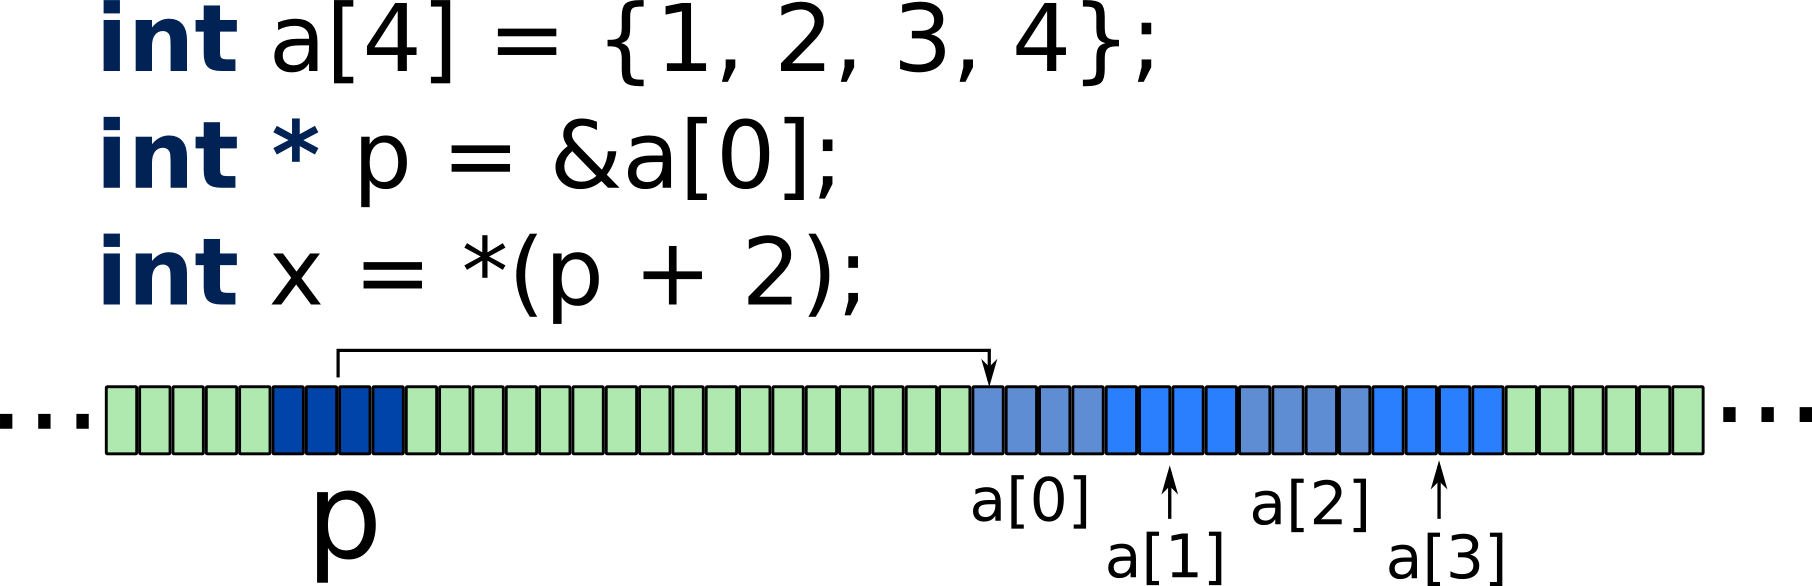
\includegraphics[width=0.95\linewidth]{images/memory_parrays_3.png}
\end{center}
\end{frame}

\begin{frame}[fragile]
\frametitle{Указатели и массивы} 
\framesubtitle{Связь массивов и указателей}
\begin{center}
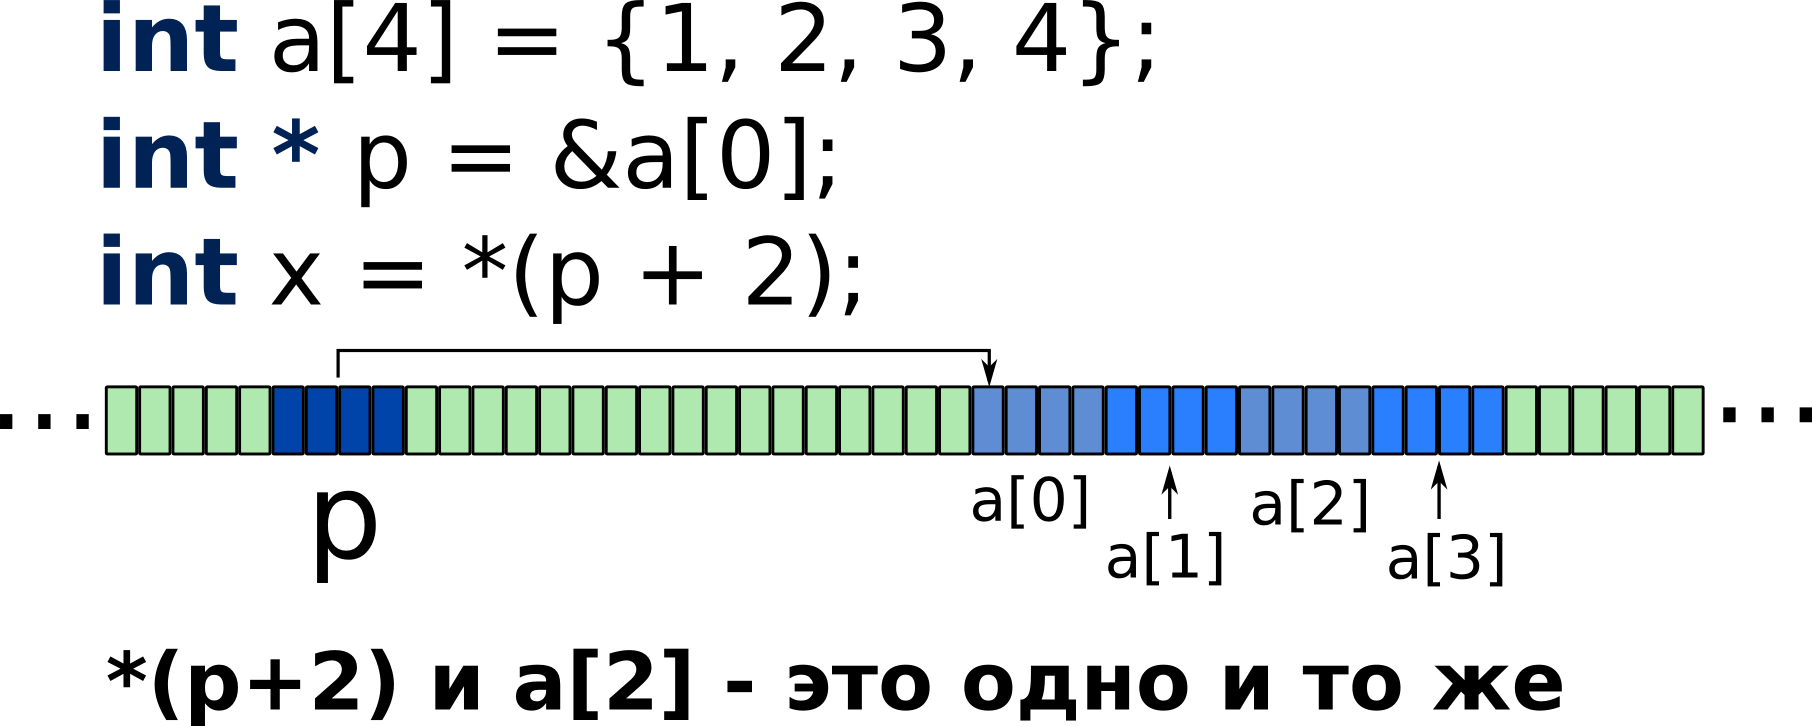
\includegraphics[width=0.95\linewidth]{images/memory_parrays_4.png}
\end{center}
\end{frame}

\begin{frame}[fragile]
\frametitle{Указатели и массивы} 
\framesubtitle{Связь массивов и указателей}
\begin{center}
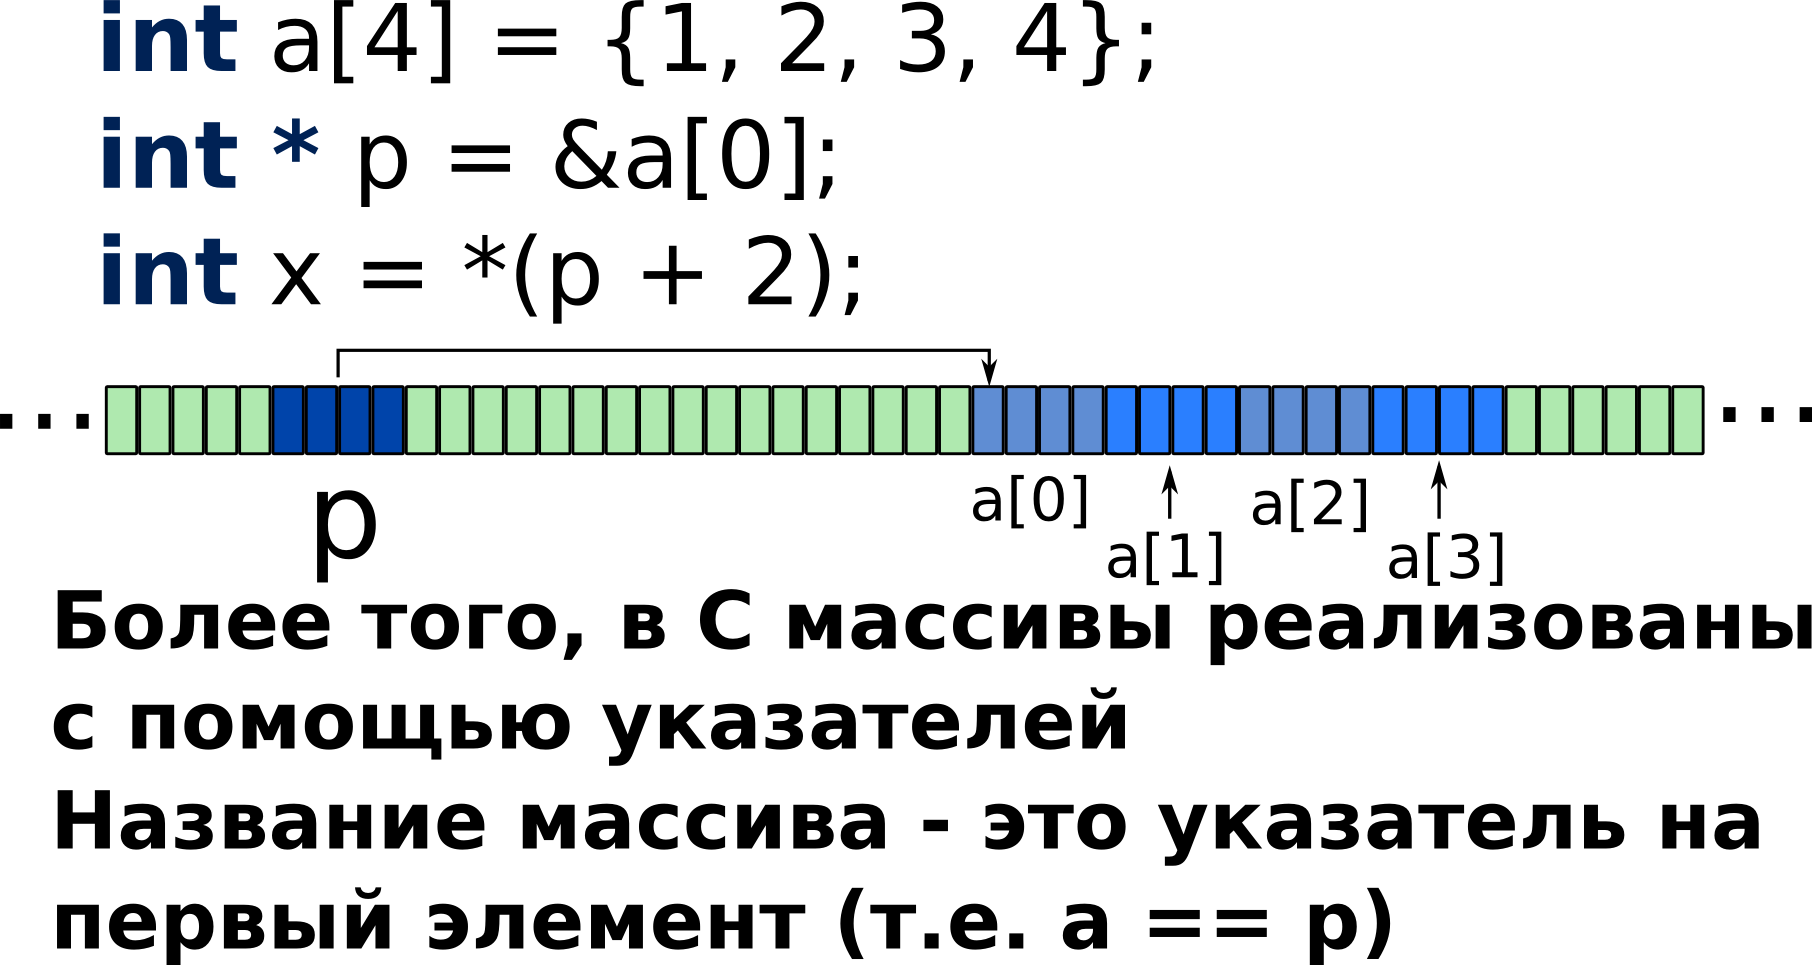
\includegraphics[width=0.95\linewidth]{images/memory_parrays_5.png}
\end{center}
\end{frame}





\section{Malloc и free. Управление памятью.}
\begin{frame}
\begin{center}
\begin{beamercolorbox}[sep=8pt,center]{part
title}
\usebeamerfont{part title}\insertsection
\end{beamercolorbox}
\end{center}
\end{frame}

\begin{frame}[fragile]
\frametitle{Управление памятью} 
\framesubtitle{Сегменты памяти процесса}
\begin{center}
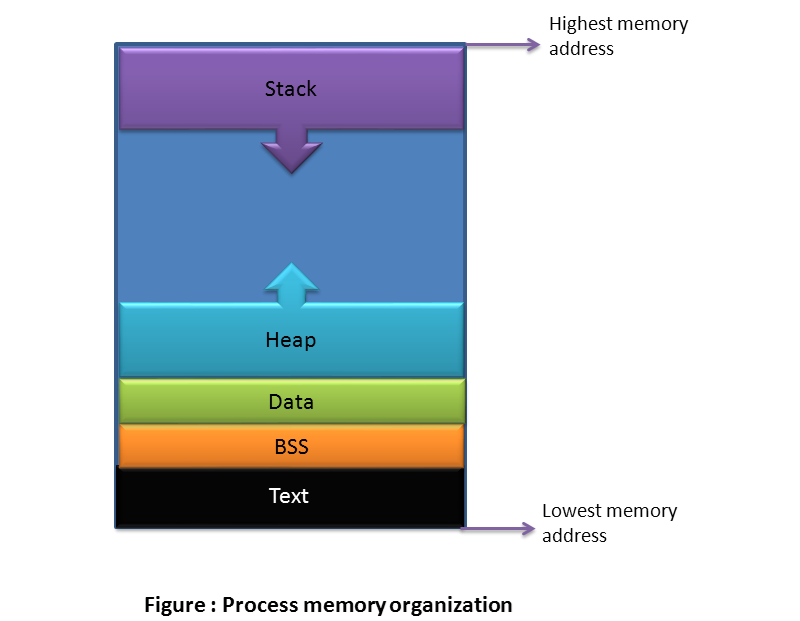
\includegraphics[width=0.8\linewidth]{images/process_memory_organization.png}
\end{center}
\end{frame}

\begin{frame}[fragile]
\frametitle{Стек (Stack)} 
\begin{itemize}
\item Стек представляет собой обычный алгоритмический стек, применённый для управления памяти
\item В нём хранятся локальные переменные
\item Имеет фиксированный размер, определяется операционной системой, на порядок меньше чем Куча
\item Немного быстрее, чем Куча
\end{itemize}
\end{frame}

\begin{frame}[fragile]
\frametitle{Куча (Heap)} 
\begin{itemize}
\item Куча представляет собой обычную алгоритмическую кучу, применённую для управления памяти
\item В ней можно динамически выделять память
\item Размер, обычно, ограничен только доступными ресурсами
\item Немного медленней, чем Стек
\end{itemize}
\end{frame}


\begin{frame}[fragile]
\frametitle{Выделение памяти в Куче с помощью malloc и free} 
\framesubtitle{Выделение памяти на 1 переменную типа int} 
\begin{center}
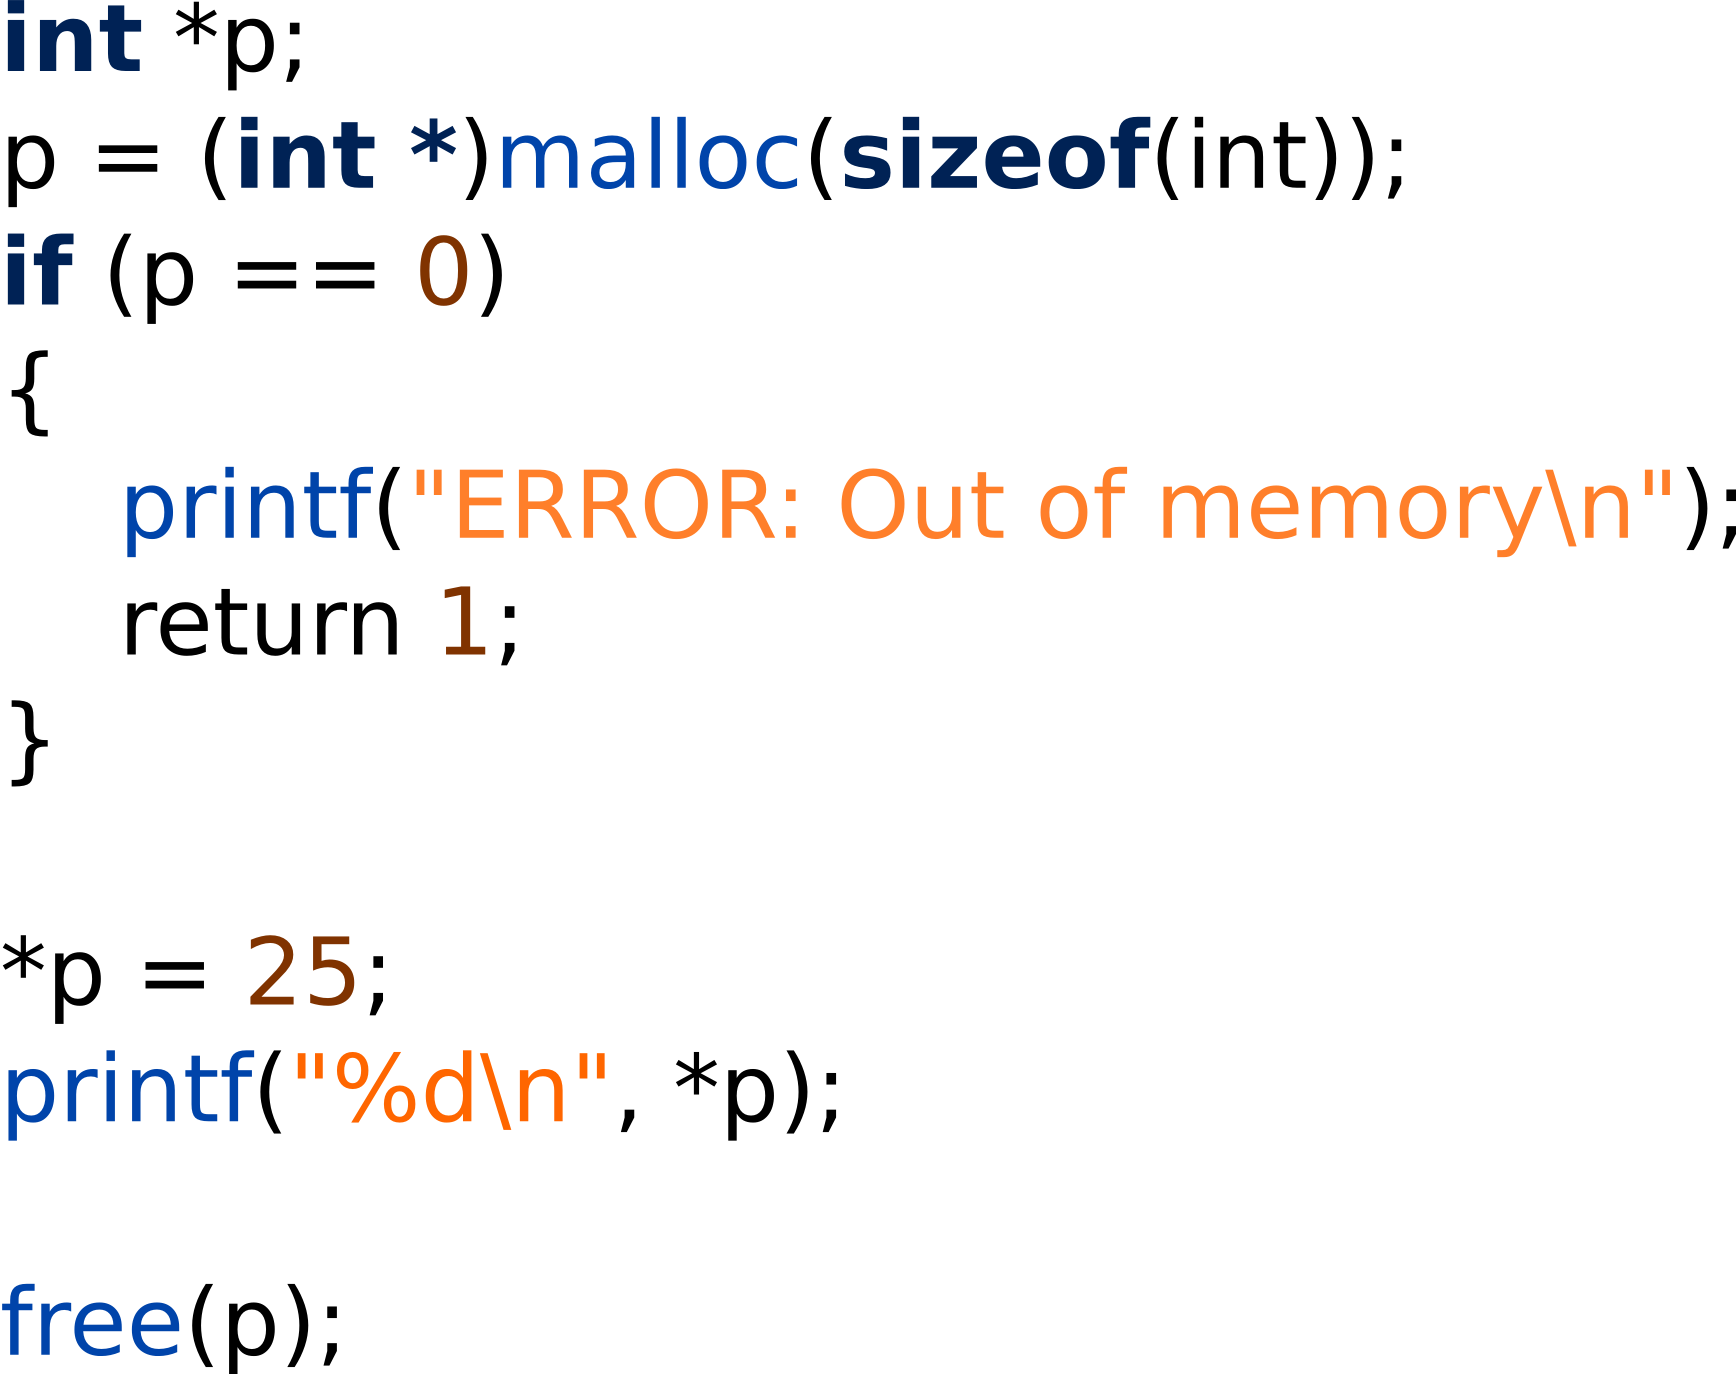
\includegraphics[width=0.55\linewidth]{images/malloc_free_1.png}
\end{center}
\end{frame}

\begin{frame}[fragile]
\frametitle{Выделение памяти в Куче с помощью malloc и free} 
\framesubtitle{Выделение памяти на массив из 100 переменных типа int} 
\begin{center}
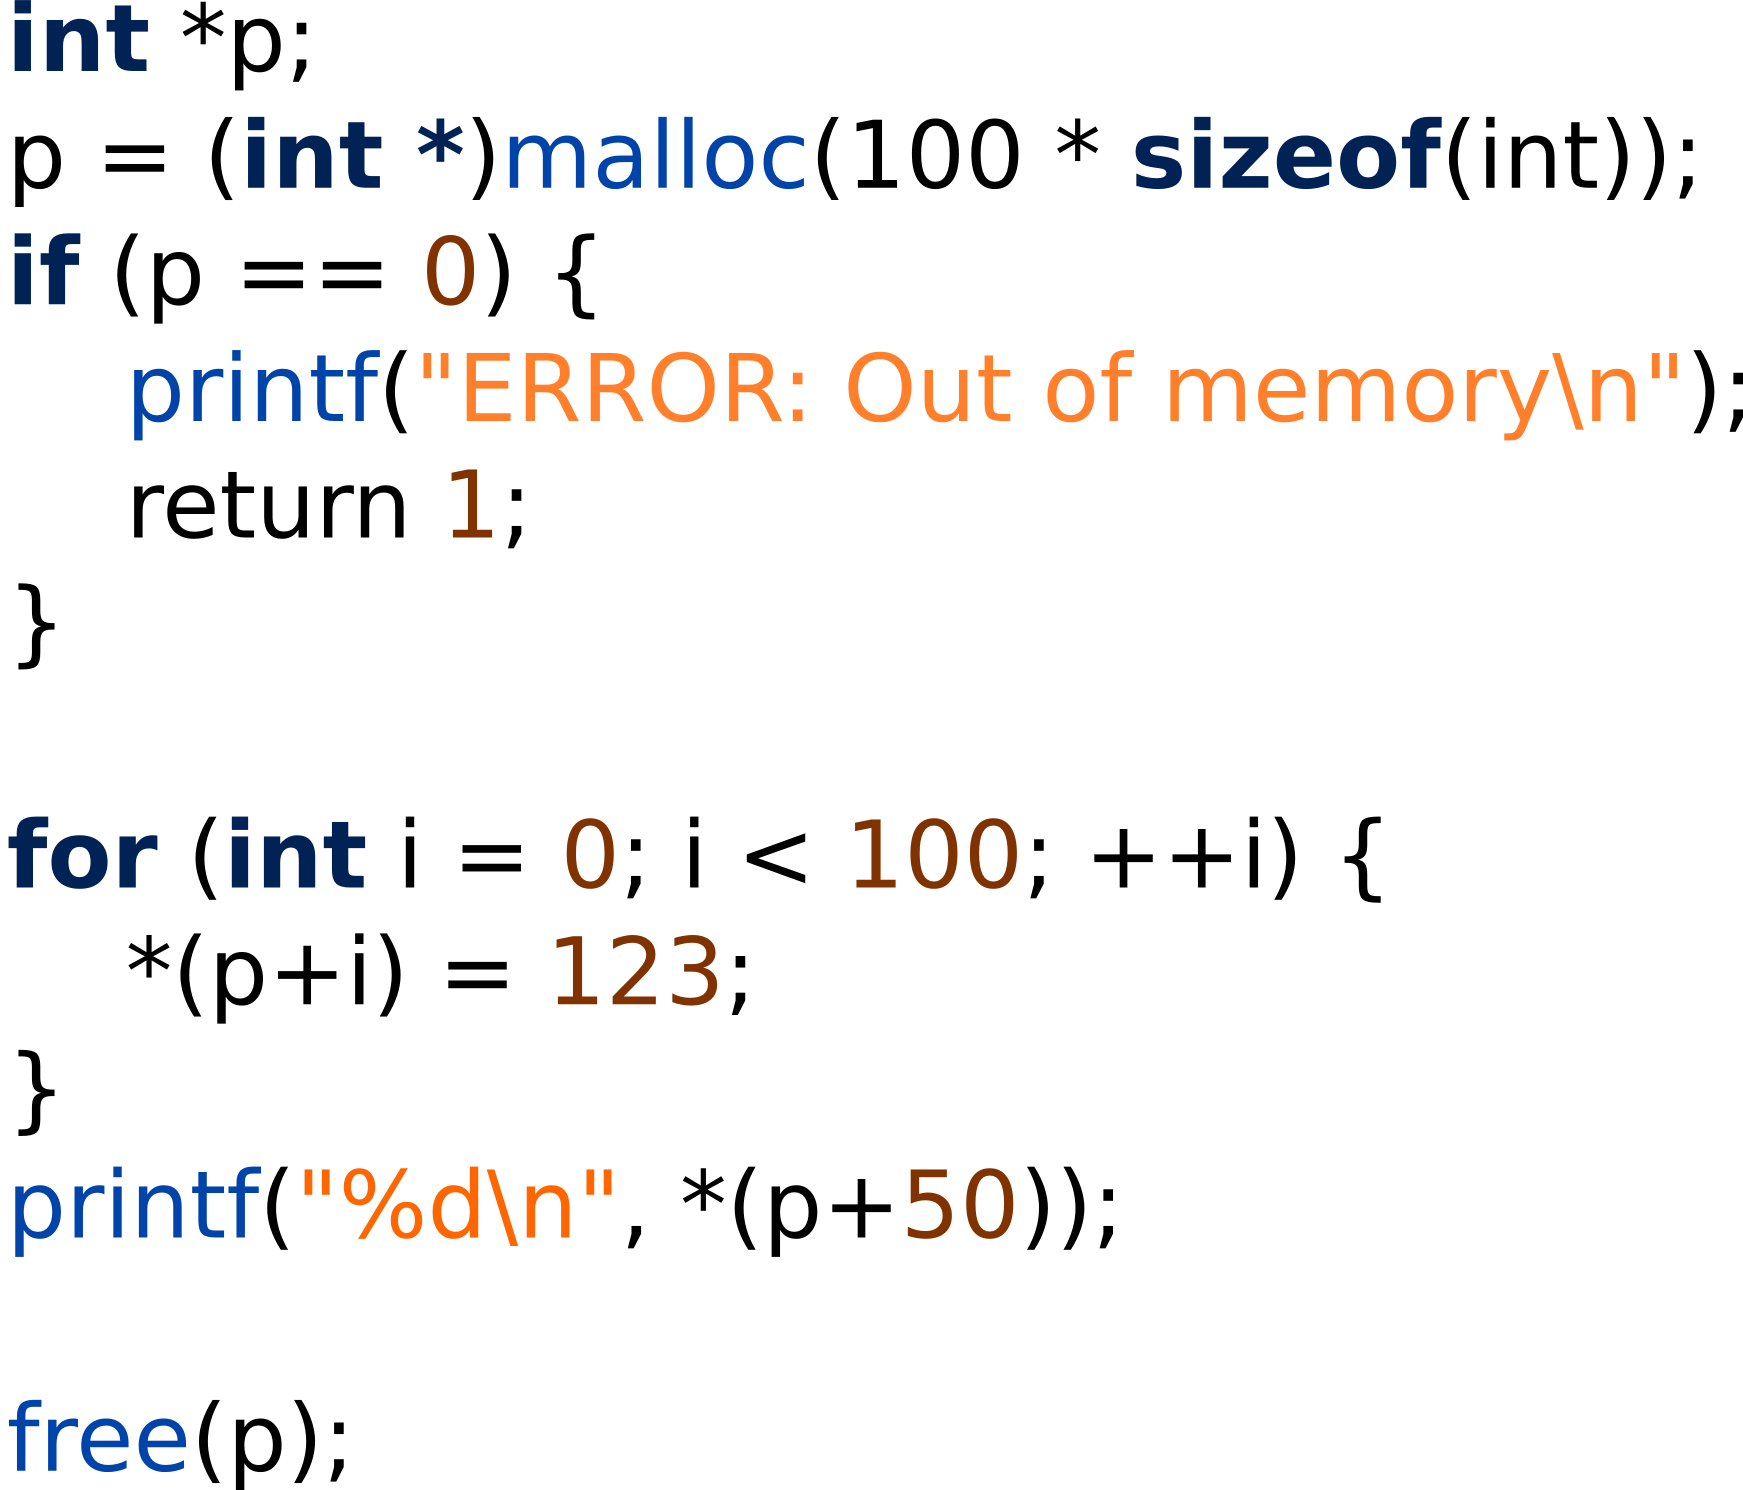
\includegraphics[width=0.55\linewidth]{images/malloc_free_2.png}
\end{center}
\end{frame}

\section{Задание}
\begin{frame}
\begin{center}
\begin{beamercolorbox}[sep=8pt,center]{part
title}
\usebeamerfont{part title}\insertsection
\end{beamercolorbox}
\end{center}
\end{frame}

\begin{frame}[fragile]
\frametitle{Задание} 
\begin{itemize}
\item Задачи на указатели -- Начинающие, Задание 2 (часть 1)
\item Задачи на структуры -- rect01
\end{itemize}
\end{frame}

\end{document}
